% Chapter discussion

\chapter{Introduction} % Main chapter title

\label{Chapter1} % For referencing the chapter elsewhere, use \ref{Chapter4} 

%----------------------------------------------------------------------------------------

% Define some commands to keep the formatting separated from the content 
\newcommand{\keyword}[1]{\textbf{#1}}
\newcommand{\tabhead}[1]{\textbf{#1}}
\newcommand{\code}[1]{\texttt{#1}}
\newcommand{\file}[1]{\texttt{\bfseries#1}}
\newcommand{\option}[1]{\texttt{\itshape#1}}

%~~~~~~~~~~~~~~~~~~~~~~~~~~~~~~~~~~~~~~~~~~~~~~~~~~~~~~~~~~~~~~~~~~~~~~~~~~~~~~~~~~~~~~~


\section {Genetic variation in humans }

No human is genetically the same as another, and this is true also for monozygotic twins that accumulate different genetic mutations or copy number variants during their life.\\ 

In the last twenty years, two main factors made possible the accurate study of the genetic variation in humans. First, in 2001 the whole genome reference sequence of humans was made publicly available to the scientific community, providing the first comprehensive description of the human genome \cite{lander2001initial, venter2001sequence}. Secondly, in the last ten years the cost of the sequencing technology decreased exponentially \cite{christensen2015assessing} (Figure \ref{fig:costPerGenome}) making possible to sequence multiple genomes, and therefore the comparisons among sequences and the identification of genetic variants (Figure \ref{fig:variantCalling} and \ref{fig:typeOfVariants}).\\  

\begin{figure}[H]
\centering
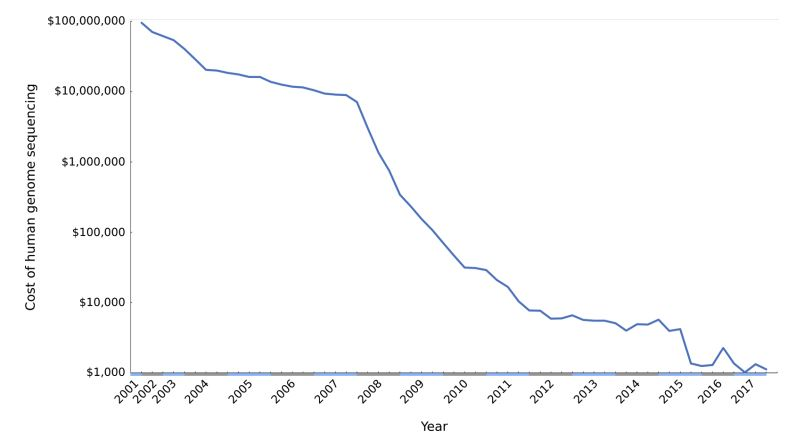
\includegraphics[width=0.7\textwidth]{fig/costPerGenome.png}
\decoRule
\caption{\textbf{Exponentially decreasing cost per Human genome, from 2009}. "\textit{Adapted from} \url{https://www.genome.gov/about-genomics/fact-sheets/Sequencing-Human-Genome-cost}"} 
\label{fig:costPerGenome}
\end{figure}

\begin{figure}[H]
\centering
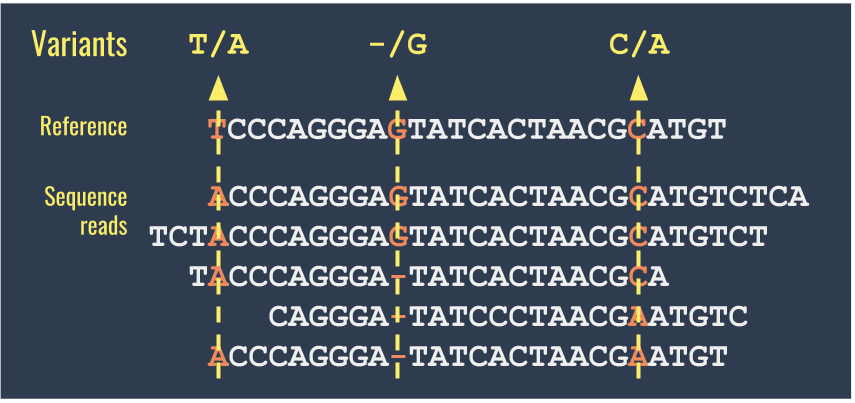
\includegraphics[width=0.7\textwidth]{fig/variantCalling.png}
\decoRule
\caption{\textbf{Variant calling} is the process of identifying genetic variants. First, sequence reads from one individual are aligned against the reference genome, then variable sites are identified as the ones where the sequence differs from the reference genome.} 
\label{fig:variantCalling}
\end{figure}

\begin{figure}[H]
\centering
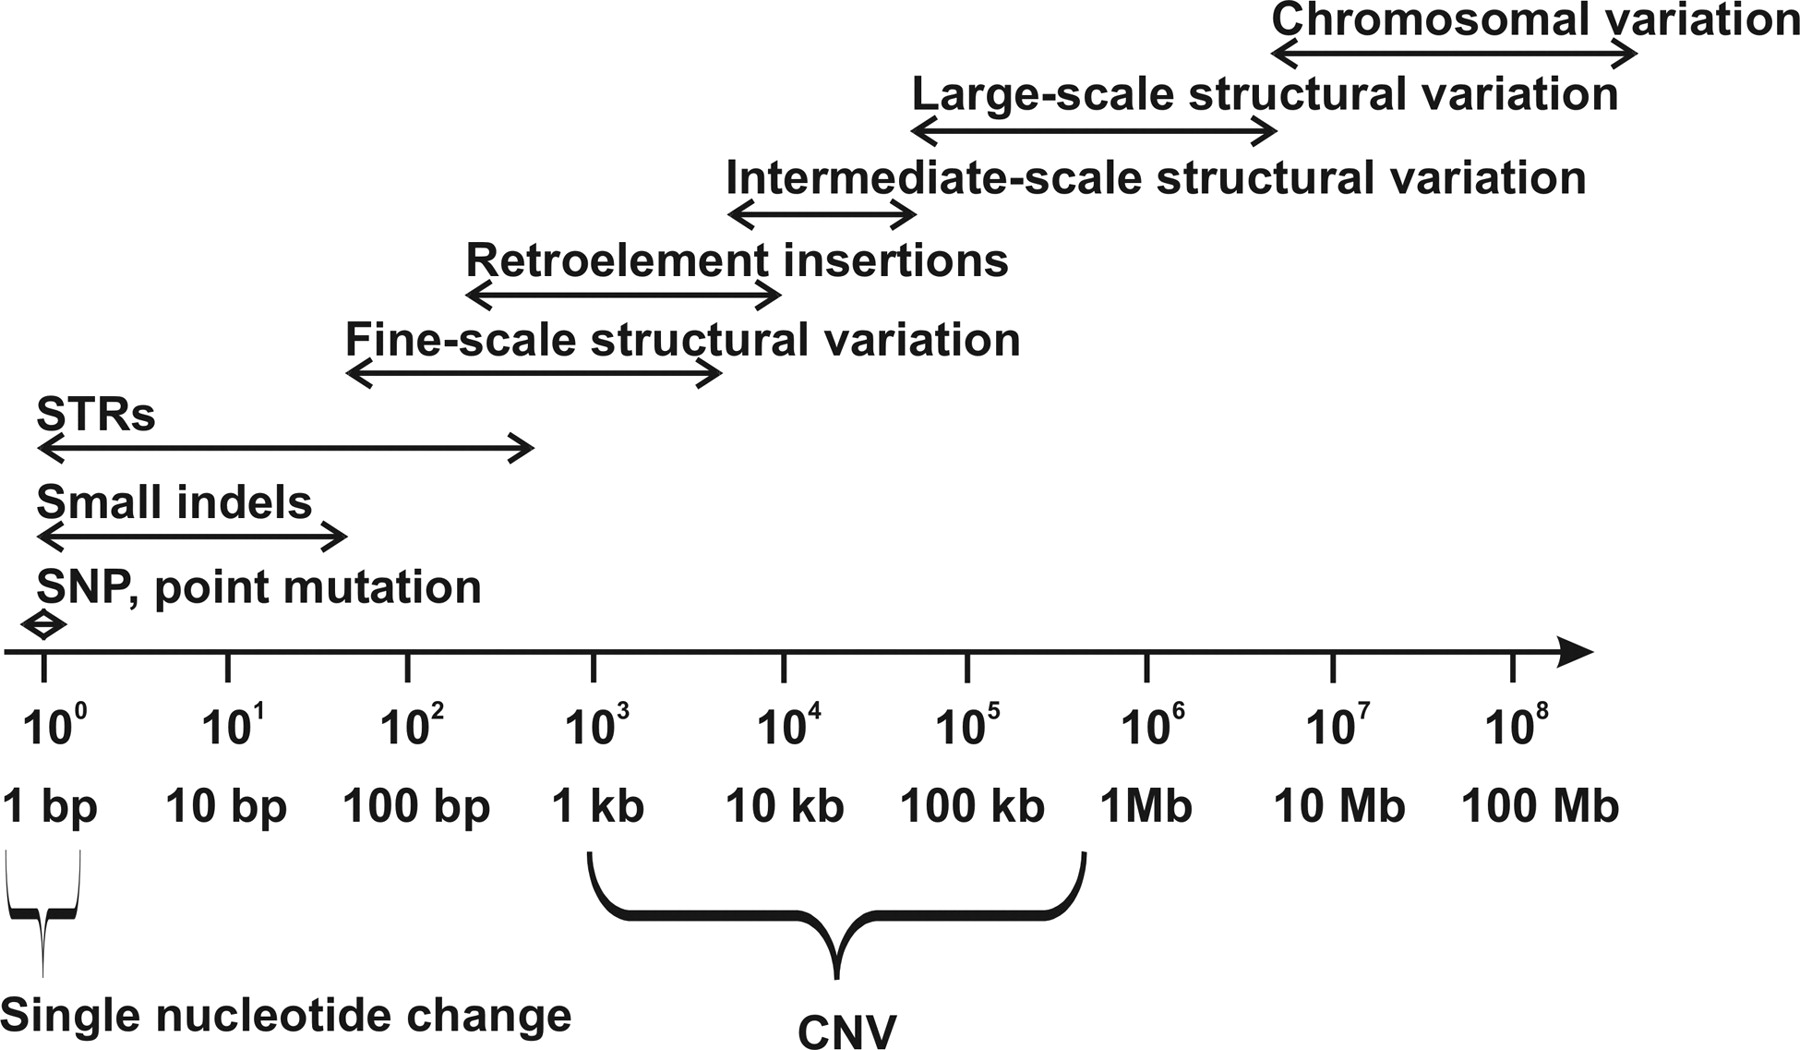
\includegraphics[width=0.7\textwidth]{fig/typeOfVariants.jpeg}
\decoRule
\caption{\textbf{Type and size of genetic variants.}"\textit{Adapted from} \cite{pollex2007copy}"} 
\label{fig:typeOfVariants}
\end{figure}

The first large-scale project that made use of whole-genome sequencing was the 1000 genomes project that used a combination of low-coverage whole-genome sequencing (WGS), deep exome sequencing, and dense microarray of 2,504 individuals from 26 populations \cite{1000genome2015global}. 
This project showed that two individuals differ at roughly  0.6\% of their genome, that corresponds at 20 millions base pairs at 4.1-5.0 million sites in a genome of 3.2 giga base (Figure \ref{fig:1000genome_grid}).\\ 

A more recent study identifies 67.3 million single-nucleotide polymorphisms (SNPs), 8.8 million small insertions or deletions (indels) and 39,997 copy number variants (CNVs) in 929 genomes. The technology used was high-coverage whole-genome sequencing (at 35X) \cite{bergstrom2019insights}. The number of variants identified by this study is comparable to the one identified by the 1000 genome project despite the lower sample size because the high-coverage sequencing increased the sensitivity. Furthermore, this study also identified 1.3 million polymorphic SNPs shared between archaic human genomes.\\

%Rare variants are more likely to derive from recent mutations, and nearly absent from genotyping array.  

%%%%%FIGURE 2.4

\begin{figure}[H]
\centering
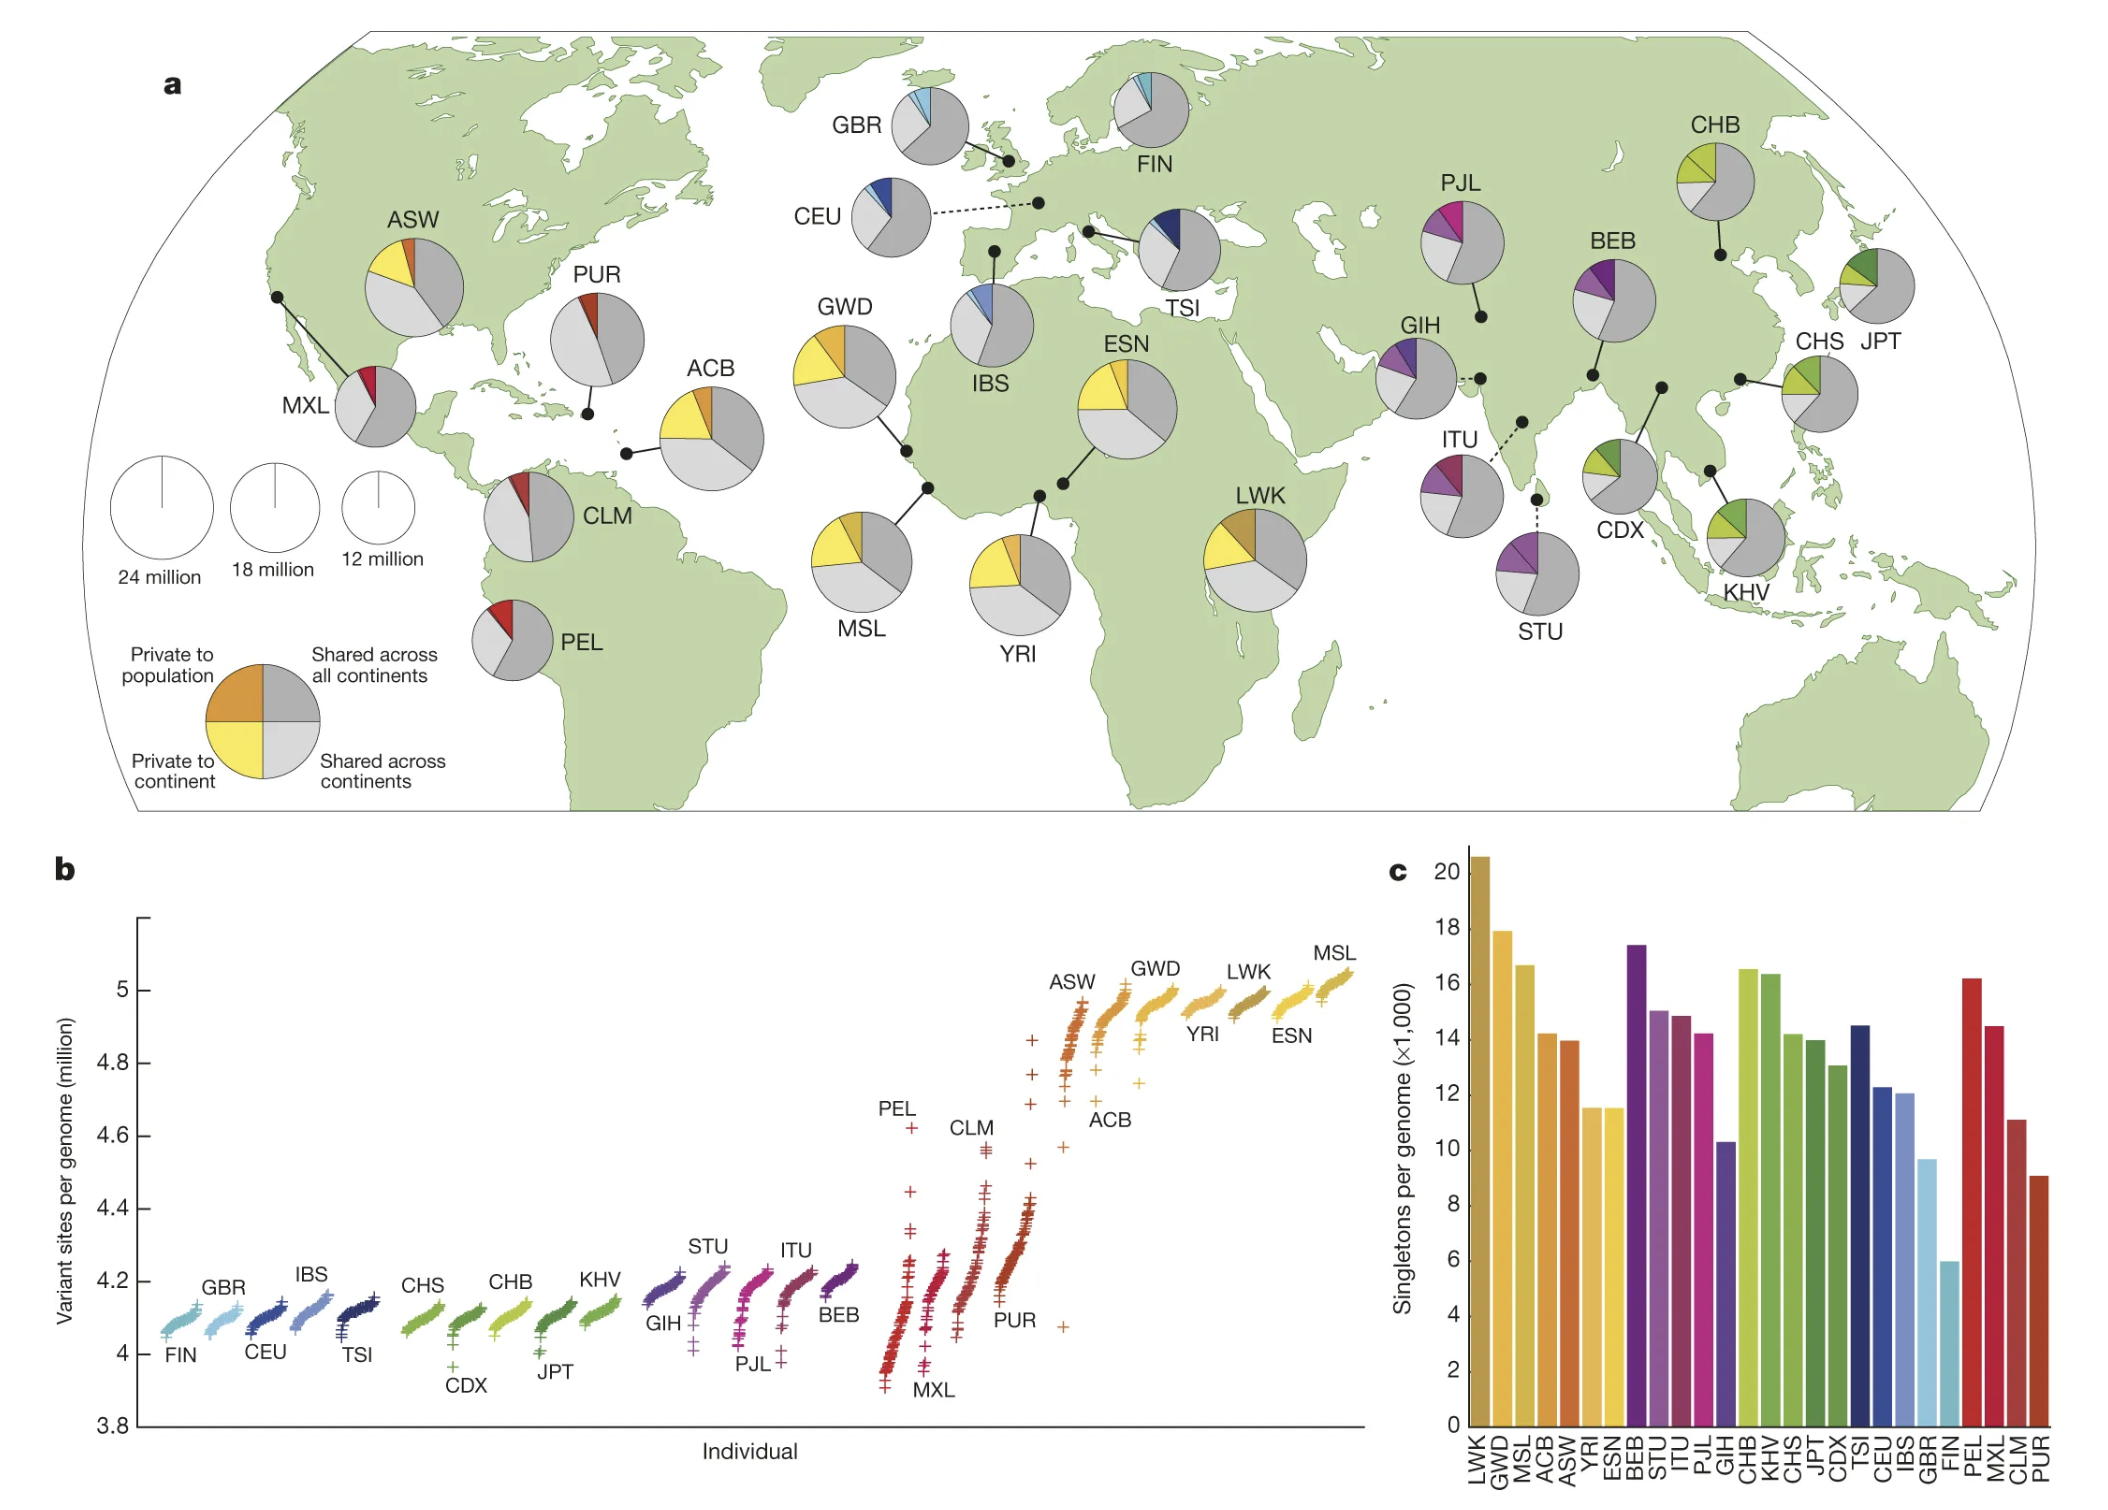
\includegraphics[width=1\textwidth]{fig/1000genome_grid.png}
\decoRule
\caption{\textbf{a}, Polymorphic variants within sampled populations. The area of each pie is proportional to the number of polymorphisms within a population. Pies are divided into four slices, representing variants private to a population (darker colour unique to population), private to a continental area (lighter colour shared across continental group), shared across continental areas (light grey), and shared across all continents (dark grey). Dashed lines indicate populations sampled outside of their ancestral continental region. \textbf{b}, The number of variant sites per genome. \textbf{c}, The average number of singletons per genome."\textit{Adapted from} \cite{1000genome2015global}}
\label{fig:1000genome_grid}
\end{figure}

%%%%%%%%%%%%%%%%%%%%%%%%%%%%%%%

\section{Genetics of miscarriages }

\subsection{Anatomy of placenta and use of the villi to extract DNA from embryos}

One week after fertilization, the blastocyst hatches from the pellucid zone and subsequently implants into the uterine wall. The placenta is a unique materno-fetal organ which begins to grow around the point of implantation and is delivered at the birth of the fetus.
The placenta has several biological functions:
\begin{itemize}
    \item \textbf{Metabolism}. The fetus takes the nutrients essential for its growth from the placenta. Some nutrients like glycogen, cholesterol, and fatty acids are synthesized in the placenta.
    \item \textbf{Transport} from and to the embryo of gases, nutrients, drugs, hormones, antibodies, wastes, and infectious agents. 
    \item \textbf{Endocrine}. After the dismission of the \textit{Corpus luteum} there is an increase of production from the placenta of human chorionic gonadotropin that is also a marker for the begin of pregnancy. Placenta also produces progesterone that helps the embryo during the implant, estrogen for proliferation and the growth of the uterus and enlargement of the breasts, human placental lactogen has structure and function similar to growth hormone and modify the metabolism of the mother to facilitate the energy supply to the fetus.
\end{itemize}

The placenta is composed of four layers that separate maternal and fetal blood \cite{placenta}:
\begin{itemize}
    \item \textbf{Syncitiotrophoblast} is the outer layer of the trophoblast and is essential for the first stage in the uterine wall invasion and homing and also establishing an interface between maternal blood and embryo. 
    \item \textbf{Cytotrophoblast} is the inner layer of the trophoblast between Syncitiotrophoblast and the external wall of the blastocyst. Contains trophoblastic stem cell. 
    \item \textbf{Villi connective tissue} is involved in the invasion of the uterine decidua and at the same time is essential to absorb nutrients from the mother for the growth of the embryo.   
    \item \textbf{Fetal capillary endothelium} is the last layer across which all exchange of gases, nutrients, hormones, and wastes occurs.
\end{itemize}

The villi are the part of the placenta that was used to extract the DNA \cite{you2008multiple} for sequencing in this project. 


\subsection{Known genetic causes of miscarriages}
%~~~~~~~~~~~~~~~ definizione 
Human reproduction is highly ineffective and it is estimated that 10-20\% of all pregnancies end in early miscarriage or early pregnancy loss (PL) during the first trimester \cite{goddijn2000genetic,zhang2009genetic} and up to 50\% of cases of recurrent pregnancy loss (RPL) do not have a clearly defined etiology \cite{practice2012evaluation}. Miscarriage is defined as the death of the fetus within 20-28 week of gestation \cite{pmid27994187, pmid25055407, pmid25944391, pmid11821293, stephenson2002cytogenetic, pmid25681385, pmid29858908}. RPL is defined as the loss of two or more consecutive pregnancies\cite{green2019review}. 
%~~~~~~~~~~~~~~~~~ consequenze aborto nella madre 
The loss of the fetus can cause physical and psychological complications to the mother, such as infection or bleeding, anxiety, guilt, and sadness. \cite{robinson2014pregnancy}.\\ 

%~~~~~~~~~~~~~~~~ cause
Miscarriages can occur for medicals or genetics causes. The most common medicals causes are infection or maternal pathology as diabetes, hypothyroidism or uterine anatomical abnormalities \cite{najafi2019chromosomal}. Mother age is an actual risk but also parental age is a risk factor in couples composed of a woman aged ≥35 years and man aged ≥40 years \cite{de2002paternal}, lifestyle is also important for pregnancy and exposure to tobacco, smoke, drug or alcohol use can be a risk factor for a miscarriage \cite{andersen2014risk}.\\

Among the genetic causes, the most common are chromosomal aneuploidies such as trisomies or deletions of large chromosomal chunks \cite{goddijn2000genetic,zhang2009genetic}. In humans, aneuploidy is the most common cause of miscarriage and can occur during mitosis in the oocytes or in sperms. The rate of aneuploidies is higher in humans (5-20\% of oocytes) than in other species (1/10,000 meiotic yeast cells, 1/2000-1/6000 Drosophila germ cells, and 1/100-1/200 murine germ cells) \cite{niakan2012human}.
Currently, it is possible to screen for aneuploidies with two methods, both invasive, chorionic villus sampling (CVS) and amniocentesis. The CVS can be made from 10 through 13 weeks’ gestation and amniocentesis is performed starting at 15 weeks’ gestation. The associated risks for a miscarriage with these two procedures are 3\% for CVS and 0.8\% for amniocentesis \cite{caughey2006chorionic}.\\

Screening for aneuploidies or other chromosomal aberration is routine prior to \textit{in vitro} fertilisation \cite{driscoll2008first}. When it is done on a miscarried fetus on DNA extracted from chorionic villi, 50-60\% of RPL cases present aneuploidies while in the remaining 40-50\% the causes are unknown \cite{pmid27994187, pmid25944391, pmid11821293, stephenson2002cytogenetic, pmid22796359, pmid22672580, pmid25681385, gaboon2013recurrent, pmid30642578}.\\


\subsection{Current knowledge of the genetic studies on miscarriages}
%~~~~~~~
The first large-scale study of miscarriage is from 2019 and was a genome-wide association study (GWAS) done on 69,118 cases from five different ancestries (trans-ethnic) for sporadic miscarriage, 750 cases of European ancestry for recurrent miscarriage, and 359,469 female has negative control \cite{laisk2019genetic}. This study identified one genome-wide significant association on chromosome 13 (rs146350366, minor allele frequency, MAF=1.2\%) for sporadic miscarriage in \textit{FGF9} responsible for the maintenance of the pregnancy and progesterone production; three genome-wide significant associations for recurrent miscarriage in chromosome 9 (rs7859844, MAF=6.4\%) chromosome 11 (rs143445068, MAF=0.8\%) and chromosome 21 (rs183453668, MAF=0.5\%). While notable for the size of the sample, this study has two main limitations. First, it is carried out on the mothers, therefore it seeks half of the possible cause of the miscarriage. Secondly, it was done using 8,664,066 markers, therefore ignoring a very large fraction of the genome. \\

Next-generation sequencing (NGS) is already used to identify mutations in fetuses with anomalies detected by ultrasound technology but is still not largely used in the study of the genetic causes of pregnancy loss. NGS is the best choice to have an adequate resolution in genetic studies. In fact, the expectation is that miscarriages depend not on a single mutation but on a combination of mutations such as compound heterozygosis \cite{qiao2016whole}. Linkage analysis on whole-exome sequences (WES) of miscarriages in two families identifies a compound heterozygous variants in \textit{DYNC2H1} (MIM 603297) at chromosome 11q22.3 in the first exon. The second family presenting two miscarriages had mutations in \textit{ALOX15} (rs113604586, rs34210653) with a minor allele frequency for all variants <1\%.\\

A recent study on 19 cases of missed abortion, uses another strategy that is filtering based on a list of 286 genes associated with early embryonic lethality and missed abortion provided by \textsc{geneontology} (GO, chordate embryonic development, cell proliferation, and forebrain development) \cite{fu2018whole}. This study identified 36 sequence variants in 32 candidate genes.\\ 

The actual use of WES in clinical analysis for the detection of variants is limited to the coding sequence to identify changes to the protein product. The successful usage of WES is due to the fact that it probably contains most (85\%) of the genes associated with diseases, the costs of the data are lower and the size is easier to manage than whole-genome sequencing \cite{rabbani2014promise}. Nevertheless, low-coverage whole-genome sequencing has already been proved useful to identifying chromosome rearrangements and copy number variants (CNVs) \cite{rajcan2019next} and it is probably the most comprehensive tool for the study of the genomic variation responsible for miscarriages since it includes also regulatory and intergenic regions. \\


\section{Project GREP}
The work I have done during my thesis is part of the project \textit{Genomics of REcurrent Pregnancy loss (GREP)} lead by the Institute of Genetics and Biophysics of the National Research Council in collaboration with the University of Napoli Federico II, and several other partners in Italy, United Kingdom, Malaysia, Pakistan, and Australia.  

GREP aims to identify genetic variants likely to cause PL not seen by current diagnostic tools (mainly comparative genomic hybridization), either because of the size or because they are located in non-coding regions not considered in medical diagnostics. The main objective of GREP is to build a predictive model that integrates genomic variation and functional annotations, based on the analysis of whole-genome sequences of miscarried embryos.\\

I participate in the data analyses of the GREP pilot project (Figure \ref{fig:projectPhases}) that includes four main stages. The first step was the collection of samples done by the University of Ferrara during 2016-2018, followed by a step of screening for euploid samples to be sequenced. Sequenced samples are being analyzed and the results will be validated using a biobank of embryonic DNA and eventually cellular models. More details will be outlined in the Result section. 

\begin{figure}[H]
\centering
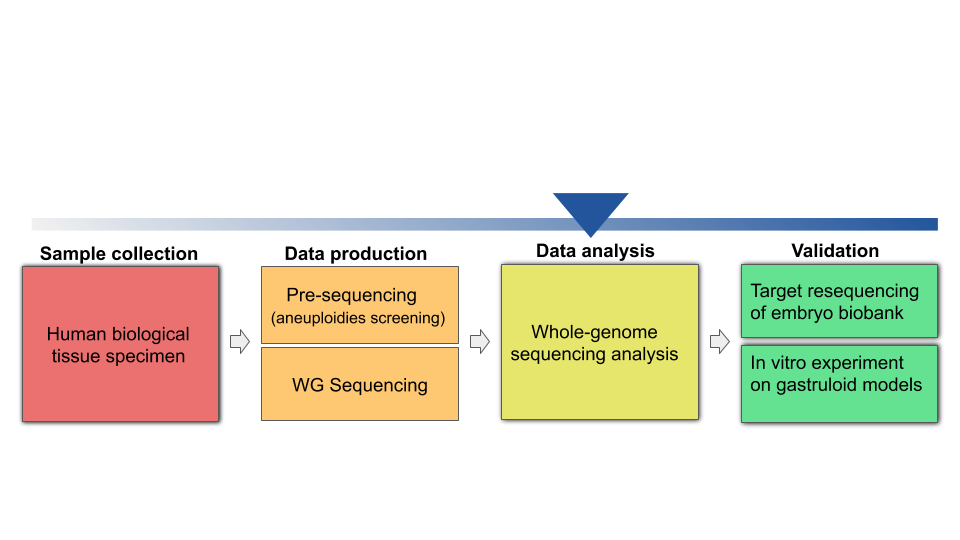
\includegraphics[width=0.80\textwidth]{fig/projectPhases.png}
\decoRule
\caption{\textbf{Pilot project phases.}} 
\label{fig:projectPhases}
\end{figure}


